\appendix
\section*{Appendix}
\section{\textit{Proof of Lemma~\ref{lem:ver}}}
\label{pro:Lemma ver}

Write Eq.~(\ref{equ:v_1}) as $P_\perp(v) = k_1mg[v/2 + \sqrt{(v^2/4 + c)}] + c_1(mg)^{3/2}$ with the shorthand $c = mg/k_2^2 > 0$ and $v = V_\perp$.
Differentiating twice, the linear term $v/2$ vanishes, the constant profile-power term $c_1(mg)^{3/2} $vanishes, and the square-root term yields

    \[ P_\perp ''(v) = k_1mg \cdot c / (4(v^2/4 + c)^{3/2}) \]

    Since $k_1$, $mg$, and $c$ are all positive, the numerator is strictly positive and the denominator is strictly positive and finite for every $v \in \mathbb{R} $.
    Hence $P_\perp''(v) > 0$ everywhere, and $P_\perp$ is strictly convex on $\mathbb{R}$.
    \qed

\section{\textit{Proof of Lemma~\ref{lem:hor}}}
\label{pro:Lemma hor}
The hovering power $P_{mh}$ is constant and does not affect the curvature.
The profile and parasite terms contribute $2c_2 > 0$ and $6c_1v \geq 0$ to the second derivative, respectively, and are therefore (strictly) convex on $v \geq 0$.
The only non-trivial part is the induced-power increment.
Substituting $u = v^2/(2v_0^2) \geq 0$ and differentiating twice gives, after simplification, the closed form

    \[ f''(v) = (1/(2v_0^2)) \cdot \phi(u),\]
    \[ \phi(u) = \frac{(2u - \sqrt{(1+u^2)}) \cdot \sqrt{(\sqrt{(1+u^2)} + u)} }{ (1+u^2)^{3/2}} \]

    The factor $\phi(u)$ vanishes at $u = 1/\sqrt{3}$ (equivalently, at $v = (2/3)^{1/4}v_0$), is positive beyond it, and is negative before it; hence the induced-power increment alone is concave near the origin, which is precisely the mathematical trace of the well-known effect that moderate forward flight relieves the induced drag.
    However, direct evaluation of the closed form shows that $\phi$ attains its global minimum at $u = 0$ with $\phi(0) = -1$, so $f''(v) \geq -1/(2v_0^2)$ for all $v \geq 0$, with equality only at $v = 0$.
    Combining all four terms,

    \begin{eqnarray*}
        P_\parallel''(v)  & = & 2c_2 + 6c_1v + P_{in}\cdot f''(v) \\ 
                    & \geq & 2c_2 - P_{in}/(2v_0^2) + 6c_1v\\ 
                    & \geq & 2c_2 - P_{in}/(2v_0^2)\\ 
                        & > & 0 
    \end{eqnarray*}

    where the last inequality follows from $4c_2v_0^2 > P_{in}$.
    Thus $P_\parallel$ is strictly convex on $v \geq 0$. 

    % \[P_\parallel''(v) = 2c_2 + 6c_1v + P_{in}\cdot f''(v) \geq\]
    %  \[2c_2 - P_{in}/(2v_0^2) + 6c_1v \geq\]
    %   \[2c_2 - P_{in}/(2v_0^2) > 0,\]

    It remains to argue that the condition $4c_2v_0^2 > P_{in}$ is not restrictive.
    First, substituting the expressions of $c_2, P_{in}$, and the momentum-theory identity $v_0^2 = W/(2n\rho A)$, the condition reduces to $(3\delta s)/(4\sqrt{C_T}) > (1+k)/\sqrt{2}$, which involves only the dimensionless aerodynamic constants of the rotor blades and is independent of the platform weight, rotor number, and disc area.
    Second, evaluated with the representative parameter set reported in~\cite{GongHao} $(W = 20 N, n = 4, \rho = 1.168 kg/m^3, A = 0.214 m^2, \delta = 0.011, s = 0.045, C_T = 0.001195, v_0 = 6.325 m/s, k = 0.11)$, the two sides evaluate to $4c_2v_0^2 \approx 111.1 W$ and $P_{in} \approx 70.2 W$, and the condition holds.
    Third, even if the condition were violated for an unconventional configuration, strict convexity would fail only in a neighbourhood of the origin: since $f''(v) \rightarrow  0$ as $v \rightarrow \infty $ while the parasite term $6c_1v$ grows linearly, there always exists a speed threshold beyond which $P_\parallel ''(v) > 0$; the non-convex region, if any, is confined to low speeds that are dominated by the hovering regime and are of limited practical interest for cruise scheduling.
    \qed

\section{\textit{Proof of Theorem~\ref{thm:optimal-range-speed}}}

\label{pro:Theorem optimal-range-speed}

Let $\mathcal{E}(d) = L \cdot LUT(\gamma)$ define the energy consumption function for a spatial displacement vector $d = (L \cos\gamma, L \sin\gamma)^T$.
Consider the energy consumption as a function of the displacement in a 2D vertical flight plane $d = (x, y)^T$, where $x = L \cos\gamma$ and $y = L \sin\gamma$.
The norm of the displacement is $r = L = \sqrt{x^2 + y^2}$ and the pitch angle is $\gamma = \arctan(y/x)$.
We define the energy functional as:

$$\mathcal{E}(x,y) = \sqrt{x^2 + y^2} \cdot LUT\left(\arctan\left(\frac{y}{x}\right)\right)$$

To establish that $\mathcal{E}(x,y)$ is convex, we examine its Hessian matrix $H$.
Let $f(\gamma) = LUT(\gamma)$.
By applying the chain rule, the first-order partial derivatives of the polar variables with respect to the Cartesian coordinates are:

$$\frac{\partial r}{\partial x} = \cos\gamma, \quad \frac{\partial r}{\partial y} = \sin\gamma, \quad \frac{\partial \gamma}{\partial x} = -\frac{\sin\gamma}{r}, \quad \frac{\partial \gamma}{\partial y} = \frac{\cos\gamma}{r}$$

The first-order partial derivatives of the energy functional $\mathcal{E} = r \cdot f(\gamma)$ are:

$$\mathcal{E}_x = \frac{\partial}{\partial x}[r f(\gamma)] = f(\gamma)\cos\gamma - f'(\gamma)\sin\gamma$$

$$\mathcal{E}_y = \frac{\partial}{\partial y}[r f(\gamma)] = f(\gamma)\sin\gamma + f'(\gamma)\cos\gamma$$

Taking the partial derivatives again to construct the Hessian matrix $H = \begin{pmatrix} \mathcal{E}_{xx} & \mathcal{E}_{xy} \\ \mathcal{E}_{yx} & \mathcal{E}_{yy} \end{pmatrix}$, we obtain:

$$\mathcal{E}_{xx} = \frac{\partial \mathcal{E}_x}{\partial \gamma}\frac{\partial \gamma}{\partial x} = -(f(\gamma) + f''(\gamma))\sin\gamma \left(-\frac{\sin\gamma}{r}\right) $$

\[= \frac{\sin^2\gamma}{r}(f(\gamma) + f''(\gamma))\]

$$\mathcal{E}_{yy} = \frac{\partial \mathcal{E}_y}{\partial \gamma}\frac{\partial \gamma}{\partial y} = (f(\gamma) + f''(\gamma))\cos\gamma \left(\frac{\cos\gamma}{r}\right) $$

\[= \frac{\cos^2\gamma}{r}(f(\gamma) + f''(\gamma))\]

$$\mathcal{E}_{xy} = \frac{\partial \mathcal{E}_x}{\partial \gamma}\frac{\partial \gamma}{\partial y} = -(f(\gamma) + f''(\gamma))\sin\gamma \left(\frac{\cos\gamma}{r}\right) $$

\[= -\frac{\sin\gamma\cos\gamma}{r}(f(\gamma) + f''(\gamma))\]

Factoring out the common terms, the Hessian matrix can be elegantly expressed as:

$$H = \frac{f(\gamma) + f''(\gamma)}{r} \begin{pmatrix} \sin^2\gamma & -\sin\gamma\cos\gamma \\ -\sin\gamma\cos\gamma & \cos^2\gamma \end{pmatrix}$$

To determine the convexity, we analyse the eigenvalues of the angular matrix $M = \begin{pmatrix} \sin^2\gamma & -\sin\gamma\cos\gamma \\ -\sin\gamma\cos\gamma & \cos^2\gamma \end{pmatrix}$.
The trace of $M$ is $Tr(M) = \sin^2\gamma + \cos^2\gamma = 1$, and its determinant is $Det(M) = \sin^2\gamma\cos^2\gamma - (-\sin\gamma\cos\gamma)^2 = 0$.
Consequently, the eigenvalues of $M$ are $0$ and $1$, which yields the eigenvalues of the full Hessian matrix $H$:

$$\lambda_1 = 0, \quad \lambda_2 = \frac{f(\gamma) + f''(\gamma)}{r}$$

The zero eigenvalue $\lambda_1$ corresponds to the radial direction, reflecting the linear scaling of energy with distance along a straight line (no curvature).
For the energy functional to be strictly convex in all tangential directions (ensuring that any angular deviation or detour incurs a strict energy penalty), the non-zero eigenvalue $\lambda_2$ must be strictly positive.
Since $r > 0$, this yields the fundamental requirement:

\begin{figure}%[]
  \centering
   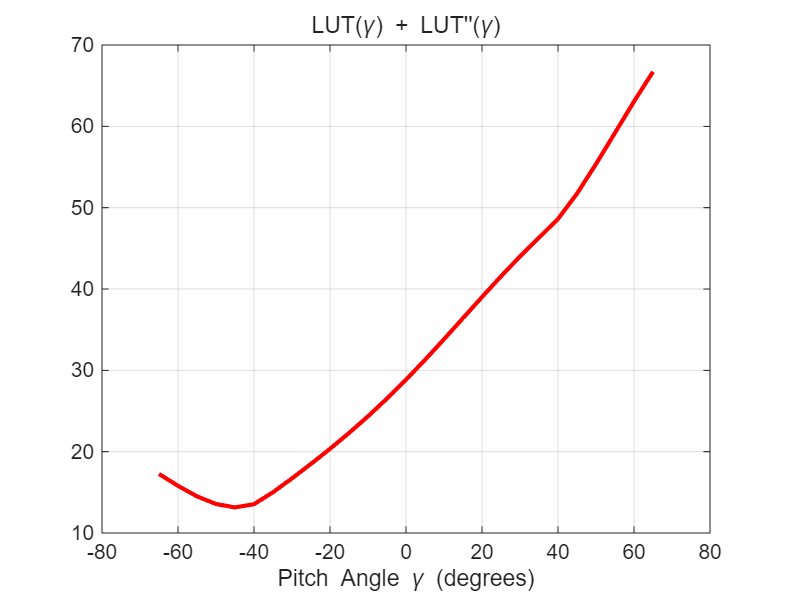
\includegraphics[width = 0.8\linewidth]{figures/lut-transition-comparison.png}
    \caption{ Shows that $LUT(\gamma)+LUT''(\gamma)$ above 0 for all pitch angles }\label{fig:LUT'+LUT''}
\end{figure}

$$f(\gamma) + f''(\gamma) > 0$$

Given that $LUT(\gamma)$ represents the optimal unit-distance energy cost, it is physically constrained to be positive, $LUT(\gamma) > 0$.
For $\mathcal{E}$ to be convex in all tangential directions, it suffices that $f(\gamma)'+f(\gamma)''>0$, which is numerically verified over the operational pitch-angle domain (Fig.~(\ref{fig:LUT'+LUT''})); for other platforms this condition can be checked offline once the LUT is constructed.

This rigorous matrix analysis confirms that the energy functional $\mathcal{E}(x,y)$ defines a strictly convex metric in the spatial field.
To bridge the theoretical gap between the strict convexity of the energy functional $\mathcal{E}(d)$ and its sub-additivity ($\mathcal{E}(d_1+d_2)<\mathcal{E}(d_1)+\mathcal{E}(d_2)$), we must first establish its positive 1-homogeneity.
For any spatial displacement vector $d$ and any positive scalar $\alpha > 0$, scaling the flight distance by $\alpha$ while maintaining the same pitch angle scales the total energy linearly.
Mathematically, this is expressed as $\mathcal{E}(\alpha d) = \|\alpha d\| \cdot LUT(\gamma) = \alpha \|d\| \cdot LUT(\gamma) = \alpha \mathcal{E}(d)$.

With both strict convexity and positive 1-homogeneity established, we can mathematically prove the strict sub-additivity for any two non-collinear displacement vectors $d_1$ and $d_2$.
Let $S = \mathcal{E}(d_1) + \mathcal{E}(d_2)$ represent the combined energy of the two independent segments.
We construct two energy-normalized vectors, $\tilde{d}_1 = \frac{d_1}{\mathcal{E}(d_1)}$ and $\tilde{d}_2 = \frac{d_2}{\mathcal{E}(d_2)}$.
Due to the 1-homogeneity, the energy of these normalized vectors is exactly unity, such that $\mathcal{E}(\tilde{d}_1) = \mathcal{E}(\tilde{d}_2) = 1$.

We define a convex combination parameter $\lambda = \frac{\mathcal{E}(d_1)}{S}$, which logically ensures $1 - \lambda = \frac{\mathcal{E}(d_2)}{S}$ and bounds the parameter within $\lambda \in (0, 1)$.
Applying the strict convexity property to these normalized vectors yields the inequality $\mathcal{E}(\lambda \tilde{d}_1 + (1-\lambda)\tilde{d}_2) < \lambda \mathcal{E}(\tilde{d}_1) + (1-\lambda)\mathcal{E}(\tilde{d}_2)$.

Substituting the definitions of $\lambda$, $\tilde{d}_1$, and $\tilde{d}_2$ into the left side of the inequality results in $\mathcal{E}\left(\frac{d_1 + d_2}{S}\right)$.
By extracting the scalar fraction $1/S$ using the 1-homogeneity property, the left side simplifies to $\frac{1}{S}\mathcal{E}(d_1 + d_2)$.
Concurrently, evaluating the right side yields $\lambda(1) + (1-\lambda)(1) = 1$.
Combining both sides produces $\frac{1}{S}\mathcal{E}(d_1 + d_2) < 1$.

Multiplying the entire expression by $S$ directly establishes the strict sub-additivity property: $\mathcal{E}(d_1 + d_2) < \mathcal{E}(d_1) + \mathcal{E}(d_2)$.
This mathematically proves that within this strictly convex spatial field, the energy required to traverse the vector sum of two non-collinear segments is strictly less than the sum of the energies required to traverse them individually.

Extending this foundational property to the continuous UAV trajectory problem, any detour path connecting the start and end points can be discretized into a sequence of $n$ spatial vectors such that $\sum_{i=1}^{n} d_i = d_{direct}$.
If at least one segment deviates from the direct geometric baseline (meaning the segments are not positively collinear), the strict sub-additivity iteratively dictates that the total energy cost of the detour strictly exceeds the direct path energy:

$$\sum_{i=1}^{n}\mathcal{E}(d_i) > \mathcal{E}\left(\sum_{i=1}^{n}d_i\right) = \mathcal{E}(d_{direct})$$

Thus, the direct straight-line path is mathematically proven to be the unique global energy minimizer.
This approach comprehensively resolves the transition optimality of gap segment by treating the energy cost as a cohesive spatial field governed by the positive definiteness of the Hessian matrix.
\qed

%%%%%%%%%%%%%%%%%%%%%%%%%%%%%%%%%%%%%%%%%%%%%%%%%%%%%%%%%%%%%%%%%%%%%%%%%%%%%%%%%%
%%%%%%%%%%%%%%%%%%%%%%%%%%%%%%%%%%%%%%%%%%%%%%%%%%%%%%%%%%%%%%%%%%%%%%%%%%%%%%%%%%
